
For this analysis all final state particles should be detected.
After $\pi^0$ decay we are going to have 4 particles: electron, proton and two photons.
The particle identification methods are applied to select the exclusive event with at least one electron, proton and two photons.

\section{Electron}
Initially electron is selected as a negative track that is identified as electron by Event Builder, i.e. has assigned pid=11.
Next we apply a series of cuts to further improve electron selection and pion rejection using the cuts from official note of "RGA analysis overview and procedures".
The code for these electron cuts has been cross checked and validated with Stefan Diehl during his $\pi^+$ SIDIS analysis cross check.
The documentation to the code used for electron PID can be found here: \href{https://drewkenjo.github.io/uconn-java-utils/annotated.html}{https://drewkenjo.github.io/uconn-java-utils/annotated.html}.

The list of electron PID cuts is following:
\begin{itemize}
	\item Event Builder PID cut: pid=11
	\item Cherenkov nphe cut
	\item DC fiducial cuts for regions 1,2,3
	\item Z vertex cut
	\item EC fiducial cut
	\item EC sampling cut
	\item minimum PCAL energy
\end{itemize}


\section{Proton}
The list of proton PID cuts is following:
\begin{itemize}
	\item Event Builder PID cut: pid=2212
	\item DC fiducial cuts for regions 1,2,3
	\item $\Delta v_z$ vertex cut
	\item {\bfseries Forward Detector} only
\end{itemize}

\section{Photon}
The list of photon PID cuts is following:
\begin{itemize}
	\item Event Builder PID cut: pid=22
	\item Forward Detector only
	\item {\bfseries not} in the sector where electron is detected
\end{itemize}


\section{Neutral pion}
In addition to individual particle PID procedures the cut on the mass of two photons is applied:
\begin{itemize}
	\item $0.07<M_{\gamma\gamma}<0.2$ GeV
\end{itemize}


\begin{figure}[hbt]
	\centering
	\includegraphics[page=6,width=0.6\linewidth]{figures/eppi0.exclusive.pdf}
	
	\caption{The distribution for mass of two photons $M_{\gamma\gamma}$}.
	\label{fig:ggmass}
\end{figure}
